\documentclass[a4paper,11pt,twoside]{article}

% Packages
\usepackage{ucs}
\usepackage[utf8x]{inputenc}
\usepackage{amsmath}
\usepackage{amsfonts}
\usepackage[francais]{babel}
\usepackage{fontenc}
\usepackage{graphicx}
\usepackage[dvips]{hyperref}
\usepackage[top=2 cm, bottom=2 cm, left=2 cm, right=2 cm]{geometry}
\renewcommand{\FrenchLabelItem}{\textbullet}
% Amélioration des environnements enumerate
\usepackage{enumerate}
\usepackage[urw-garamond]{mathdesign}
\usepackage{concmath}
\usepackage{commath}
\usepackage{color}
\usepackage{pgf}
\usepackage{siunitx}
\usepackage{ifthen}
\usepackage{color}

\definecolor{mygreen}{rgb}{0,0.6,0}
\definecolor{mygray}{rgb}{0.5,0.5,0.5}
\definecolor{mymauve}{rgb}{0.58,0,0.82}
\usepackage{listings}
\lstset{ %
  backgroundcolor=\color{white},   % choose the background color; you must add \usepackage{color} or \usepackage{xcolor}
  basicstyle=\small,        % the size of the fonts that are used for the code
  breakatwhitespace=false,         % sets if automatic breaks should only happen at whitespace
  breaklines=true,                 % sets automatic line breaking
  captionpos=b,                    % sets the caption-position to bottom
  commentstyle=\color{mygreen},    % comment style
  deletekeywords={...},            % if you want to delete keywords from the given language
  escapeinside={\%*}{*)},          % if you want to add LaTeX within your code
  extendedchars=true,              % lets you use non-ASCII characters; for 8-bits encodings only, does not work with UTF-8
  frame=single,                    % adds a frame around the code
  keepspaces=true,                 % keeps spaces in text, useful for keeping indentation of code (possibly needs columns=flexible)
  keywordstyle=\color{blue},       % keyword style
  language=Python,                 % the language of the code
  morekeywords={*,...},            % if you want to add more keywords to the set
  numbers=left,                    % where to put the line-numbers; possible values are (none, left, right)
  numbersep=5pt,                   % how far the line-numbers are from the code
  numberstyle=\tiny\color{mygray}, % the style that is used for the line-numbers
  rulecolor=\color{black},         % if not set, the frame-color may be changed on line-breaks within not-black text (e.g. comments (green here))
  showspaces=false,                % show spaces everywhere adding particular underscores; it overrides 'showstringspaces'
  showstringspaces=false,          % underline spaces within strings only
  showtabs=false,                  % show tabs within strings adding particular underscores
  stepnumber=2,                    % the step between two line-numbers. If it's 1, each line will be numbered
  stringstyle=\color{mymauve},     % string literal style
  tabsize=2,                       % sets default tabsize to 2 spaces
  title=\lstname                   % show the filename of files included with \lstinputlisting; also try caption instead of title
}

\setlength\parindent{0pt}

\newcommand{\HRule}{\rule{\linewidth}{0.35mm}}
\setlength{\fboxrule}{.5mm}
\author{L. Charleux}
\title{Oscillateurs}

\date{}

\begin{document}

\maketitle


\begin{figure}[t]
\begin{center}
\input{oscillator_structure.pdf_tex}
\end{center}
\caption{Modélisation de l'oscillateur non linéaire utilisé: une masse $m$ est excitée par un déplacement  $x_d$ au travers d'une raideur variable $k(x)$ et d'un amortissement fixe $\mu$.}
\label{fig:oscillator_structure}
\end{figure}

\section*{Introduction}

\noindent Ce document rassemble quelques idées sur les oscillateurs non linéaires destinés à récupérer de l'énergie vibratoire. Le code Python associé est disponible sous GitHub ici : \url{https://github.com/lcharleux/oscillators}. Pour le moment, il est public et libre ce qui facilite nos discussions mais je peux le rendre privé.

\section{Formulation du problème}

\noindent On considère l'oscillateur représenté sur la figure \ref{fig:oscillator_structure}. Celui-ci est non linéaire du fait de la raideur variable $k(x)$. Pour simplifier la construction de cette raideur nous choisissons de raisonner en terme d'énergie potentielle $\mathcal E_p(x)$. La force appliquée par la raideur sur la masse mobile est alors $F_k(x) = -\frac{d\mathcal E_p}{dt}(x)$. Le problème prend la forme suivant:

\begin{equation}
\ddot{x} = -\frac{\mu}{m} \dot{x} - \frac{1}{m}\frac{d\mathcal E_p}{dx}(x) - \ddot{x}_d
\end{equation}



\noindent  On réduit le problème en introduisant:
\begin{itemize}
\item L'amortissement massique $a = \mu / m$.
\item L'énergie potentielle massique $e_p(x) = \mathcal E_p(x) / m$

\end{itemize}


Le problème prend alors la forme suivante:

\begin{equation}
\ddot{x} = -a \dot{x} - \frac{d e_p}{dx}(x) - \ddot{x}_d
\end{equation}

Enfin, on peut reformuler l'équation scalaire du second ordre en une équation vectorielle du premier ordre comme suit. On pose:

$$
X = \begin{bmatrix}
x \\
\dot x
\end{bmatrix}
$$

Alors:

$$
\dot X = \begin{bmatrix}
\dot x \\
\ddot x
\end{bmatrix}
=
\begin{bmatrix}
\dot x \\
-a \dot{x} -\frac{de_p}{dx}(x) -\ddot{x}_d
\end{bmatrix}
$$

Cette formulation est nécessaire car utilisée par les solveurs dédiés aux équations différentielles.

\section{Performance énergétique du système}
 
\noindent  L'énergie massique $e$ de l'oscillateur à un instant donné est la somme de l'énergie potentielle massique $e_p$ et de l'énergie cinétique massique $e_p = \frac{1}{2} \dot{x}^2$. Dans ce qui suite on s'intéresse à un régime établi au sens énergétique, c'est-à-dire:

\begin{equation}
\frac{de}{dt} = 0
\end{equation}

\noindent  Dans ce cas, il a égalité entre l'énergie prélevée par le système et celle qu'il perd au travers de l'amortissement\footnote{qui représente à la fois l'amortissement physique réel du système et l'amortissement induit par la charge du générateur.}. On peut donc caractériser la performance du système par la puissance massique moyenne consommée par l'amortissement $\bar p_a$:

\begin{equation}
\bar p_a = \frac{a}{T}\int_0^T \dot{x}^2 dt 
\end{equation}

\section{Oscillateur linéaire}

L'oscillateur linéaire a valeur d'élément de comparaison. Il est un cas particulier du problème considéré car:

\begin{equation}
e_p = \frac{\omega_0^2}{2} x^2
\end{equation}

Le problème se ramène alors à résoudre:

\begin{equation}
\ddot{x} = -a \dot{x} - \omega_0^2 x - \ddot{x}_d
\end{equation}

\subsection{Régime établie avec excitation sinusoïdale}

\begin{figure}
\begin{center}
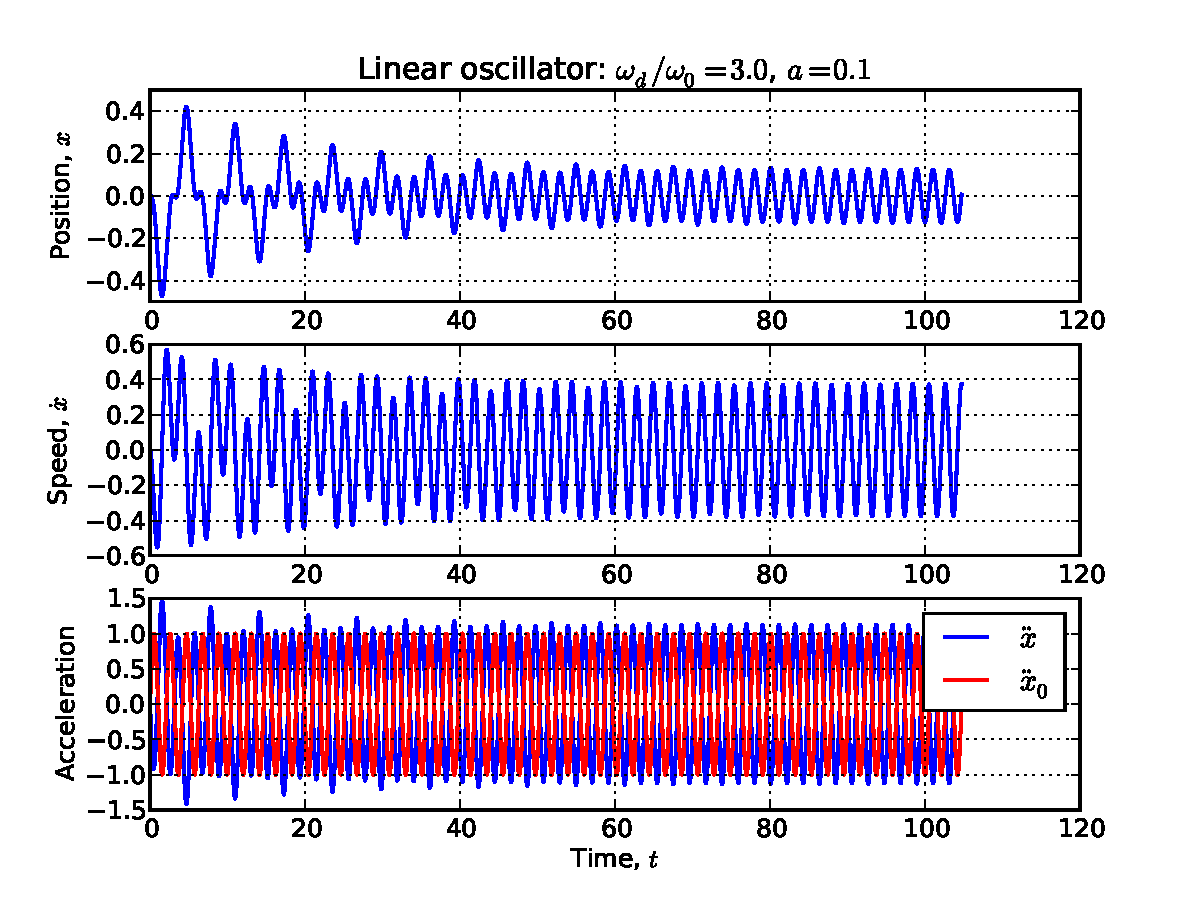
\includegraphics[width = 1.\textwidth]{../oscillators/example_code/linear_oscillator_signal.pdf}
\end{center}
\caption{Simulation du régime transitoire et de la convergence vers le régime établi dans le cas d'un oscillateur linéaire amorti (\href{https://github.com/lcharleux/oscillators/blob/master/oscillators/example_code/linear_oscillator_demo.py}{code}).}
\label{fig:linear_oscillator_power}
\end{figure}

\begin{figure}
\begin{center}
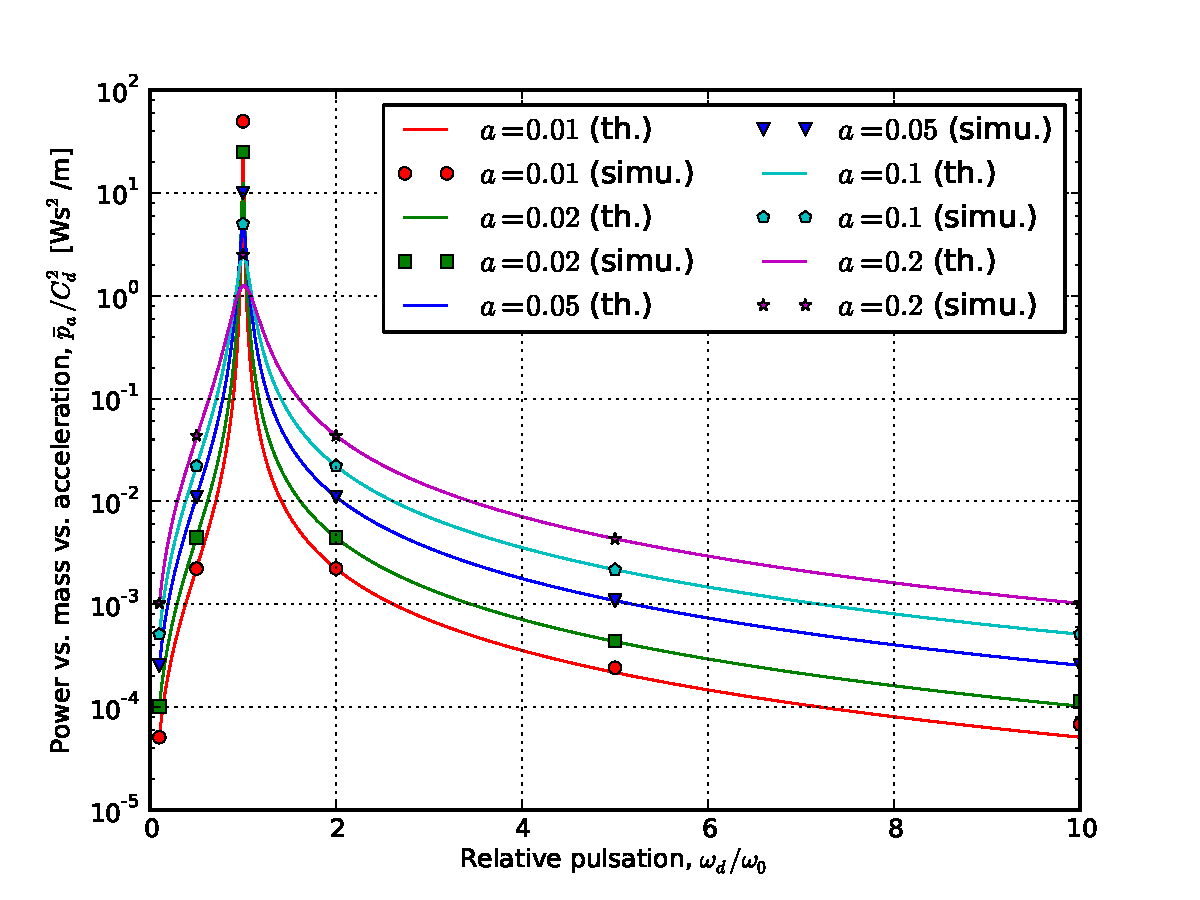
\includegraphics[width = 1.\textwidth]{../oscillators/example_code/linear_oscillator_power.pdf}
\end{center}
\caption{Power harvesting capability of the linear oscillator: confrontation of numerical simulations with the theory (\href{https://github.com/lcharleux/oscillators/blob/master/oscillators/example_code/linear_oscillator_power.py}{code}).}
\label{fig:linear_oscillator_power}
\end{figure}

On suppose que :
$$
x_d(t) = A_d \sin(\omega_d t)
$$

La solution du problème est:

\begin{equation}
x(t) = A \sin(\omega_d t + \phi) 
\end{equation}

Avec:
\begin{equation}
A = A_d\dfrac{\omega_d^2 }{\sqrt{\omega_d^2 a^2 + \left( \omega_0^2 - \omega_d^2\right)^2 } } 
\end{equation}

Et:

\begin{equation}
\phi = \arctan \left(\dfrac{a\omega_d}{\omega_d^2 - \omega_0^2} \right )
\end{equation}

La puissance massique moyenne en régime établi est donc:

\begin{equation}
\bar p_a = \frac{a\omega_d^2 A^2}{2} =   \dfrac{ a A_d^2 \omega_d^6}{2\left(a^2\omega_d^2 + \left( \omega_0^2 - \omega_d^2\right)^2 \right) } 
\end{equation}

On va s'intéresser au cas où l'accélération $\ddot{x}_d$ est une constante, on pose donc $A_d = C_d / \omega_d^2$, on a alors:

\begin{equation}
\bar p_a = \dfrac{ a C_d^2 \omega_d^2}{2\left(a^2\omega_d^2 + \left( \omega_0^2 - \omega_d^2\right)^2 \right) } 
\end{equation}

Les performances du système pour une accélération d'excitation constante alors données par:

\begin{equation}
\dfrac{\bar p_a}{C_d^2} = \dfrac{ a \omega_d^2}{2\left(a^2\omega_d^2 + \left( \omega_0^2 - \omega_d^2\right)^2 \right) } 
\end{equation}

La figure \ref{fig:linear_oscillator_power} montre que les résultats des simulations numériques sont en excellent accord avec la théorie.

\end{document}
